\documentclass{article}
\usepackage{framed}
\usepackage{scrextend}
\usepackage{xcolor}
\usepackage[spanish,es-tabla]{babel}
\usepackage[dvips,a3paper,centering,margin=2cm]{geometry}
\usepackage{multicol}
\usepackage{subcaption}
\usepackage[utf8]{inputenc}
\usepackage{color}
\usepackage{float}
\usepackage{cite}
\usepackage{colortbl}
\usepackage{tabulary}
\usepackage{multirow}
\usepackage{amsmath}
\usepackage{graphicx}
\usepackage[breaklinks=true,hidelinks]{hyperref}
\definecolor{shadecolor}{RGB}{26, 147, 111}
\definecolor{rb}{rgb}{0.025,0.5,0.9} 
\definecolor{na}{rgb}{0.8274,0.305,0.196} 
\definecolor{title}{RGB}{26, 147, 111}
\definecolor{ver}{RGB}{255,255,255}
\pagestyle{empty}
\def\to{\rightarrow}
\begin{document}
\vspace*{-2cm}
\changefontsizes{14pt}
\hspace*{-1cm}
\begin{minipage}{0.2\linewidth}
\vspace{0.7cm}
\vspace*{-0.15cm}
\includegraphics[scale=0.12]{images/ifir.eps}
\end{minipage}
\vspace*{-0.4cm}
\begin{minipage}{0.6\linewidth}
\vspace*{0.7cm}
\begin{center}
\changefontsizes{15pt}
\hspace*{-0.1cm}
\textbf{\textcolor{title}{Análisis del PM\textsubscript{10} medido y el AOD\textsubscript{550nm} estimado a partir de las mediciones de irradiancia solar VIS-NIR en el Área Metropolitana de Monterrey}}
\end{center}
\vspace{-1cm}
\begin{center}
\changefontsizes{11pt}
Gamaliel López-Padilla\textsuperscript{\ref{fcfm}}, Adriana Ipiña\textsuperscript{\ref{IFIR}}, Constanza Zuñiga Villareal\textsuperscript{\ref{fcfm}},Rubén Piacentini\textsuperscript{\ref{IFIR}}\\
\begin{enumerate}
    \centering
    \vspace{-0.25cm}
    \item Facultad de Ciencias Físico-Matemáticas,UANL, México \label{fcfm} \vspace{-0.25cm}
    \item Instituto de Física Rosario,CONICET-UNR, Argentina \label{IFIR} \vspace{-0.25cm}
\end{enumerate}
email: giovannilopez9808@gmail.com, ipina@ifir-conicet.gov.ar
\end{center}
\end{minipage}
\begin{minipage}{0.2\linewidth}
\hspace*{0.2cm}

\includegraphics[scale=0.2]{images/fcfm.eps}
\end{minipage}
\vspace{0.2cm}
\changefontsizes{12pt}
\begin{center}
\begin{shaded}
\textbf{\textcolor{ver}{Introducción}}
\end{shaded}
\end{center}
\vspace*{-0.5cm}
\begin{minipage}{0.4\linewidth}
\begin{figure}[H]
\centering
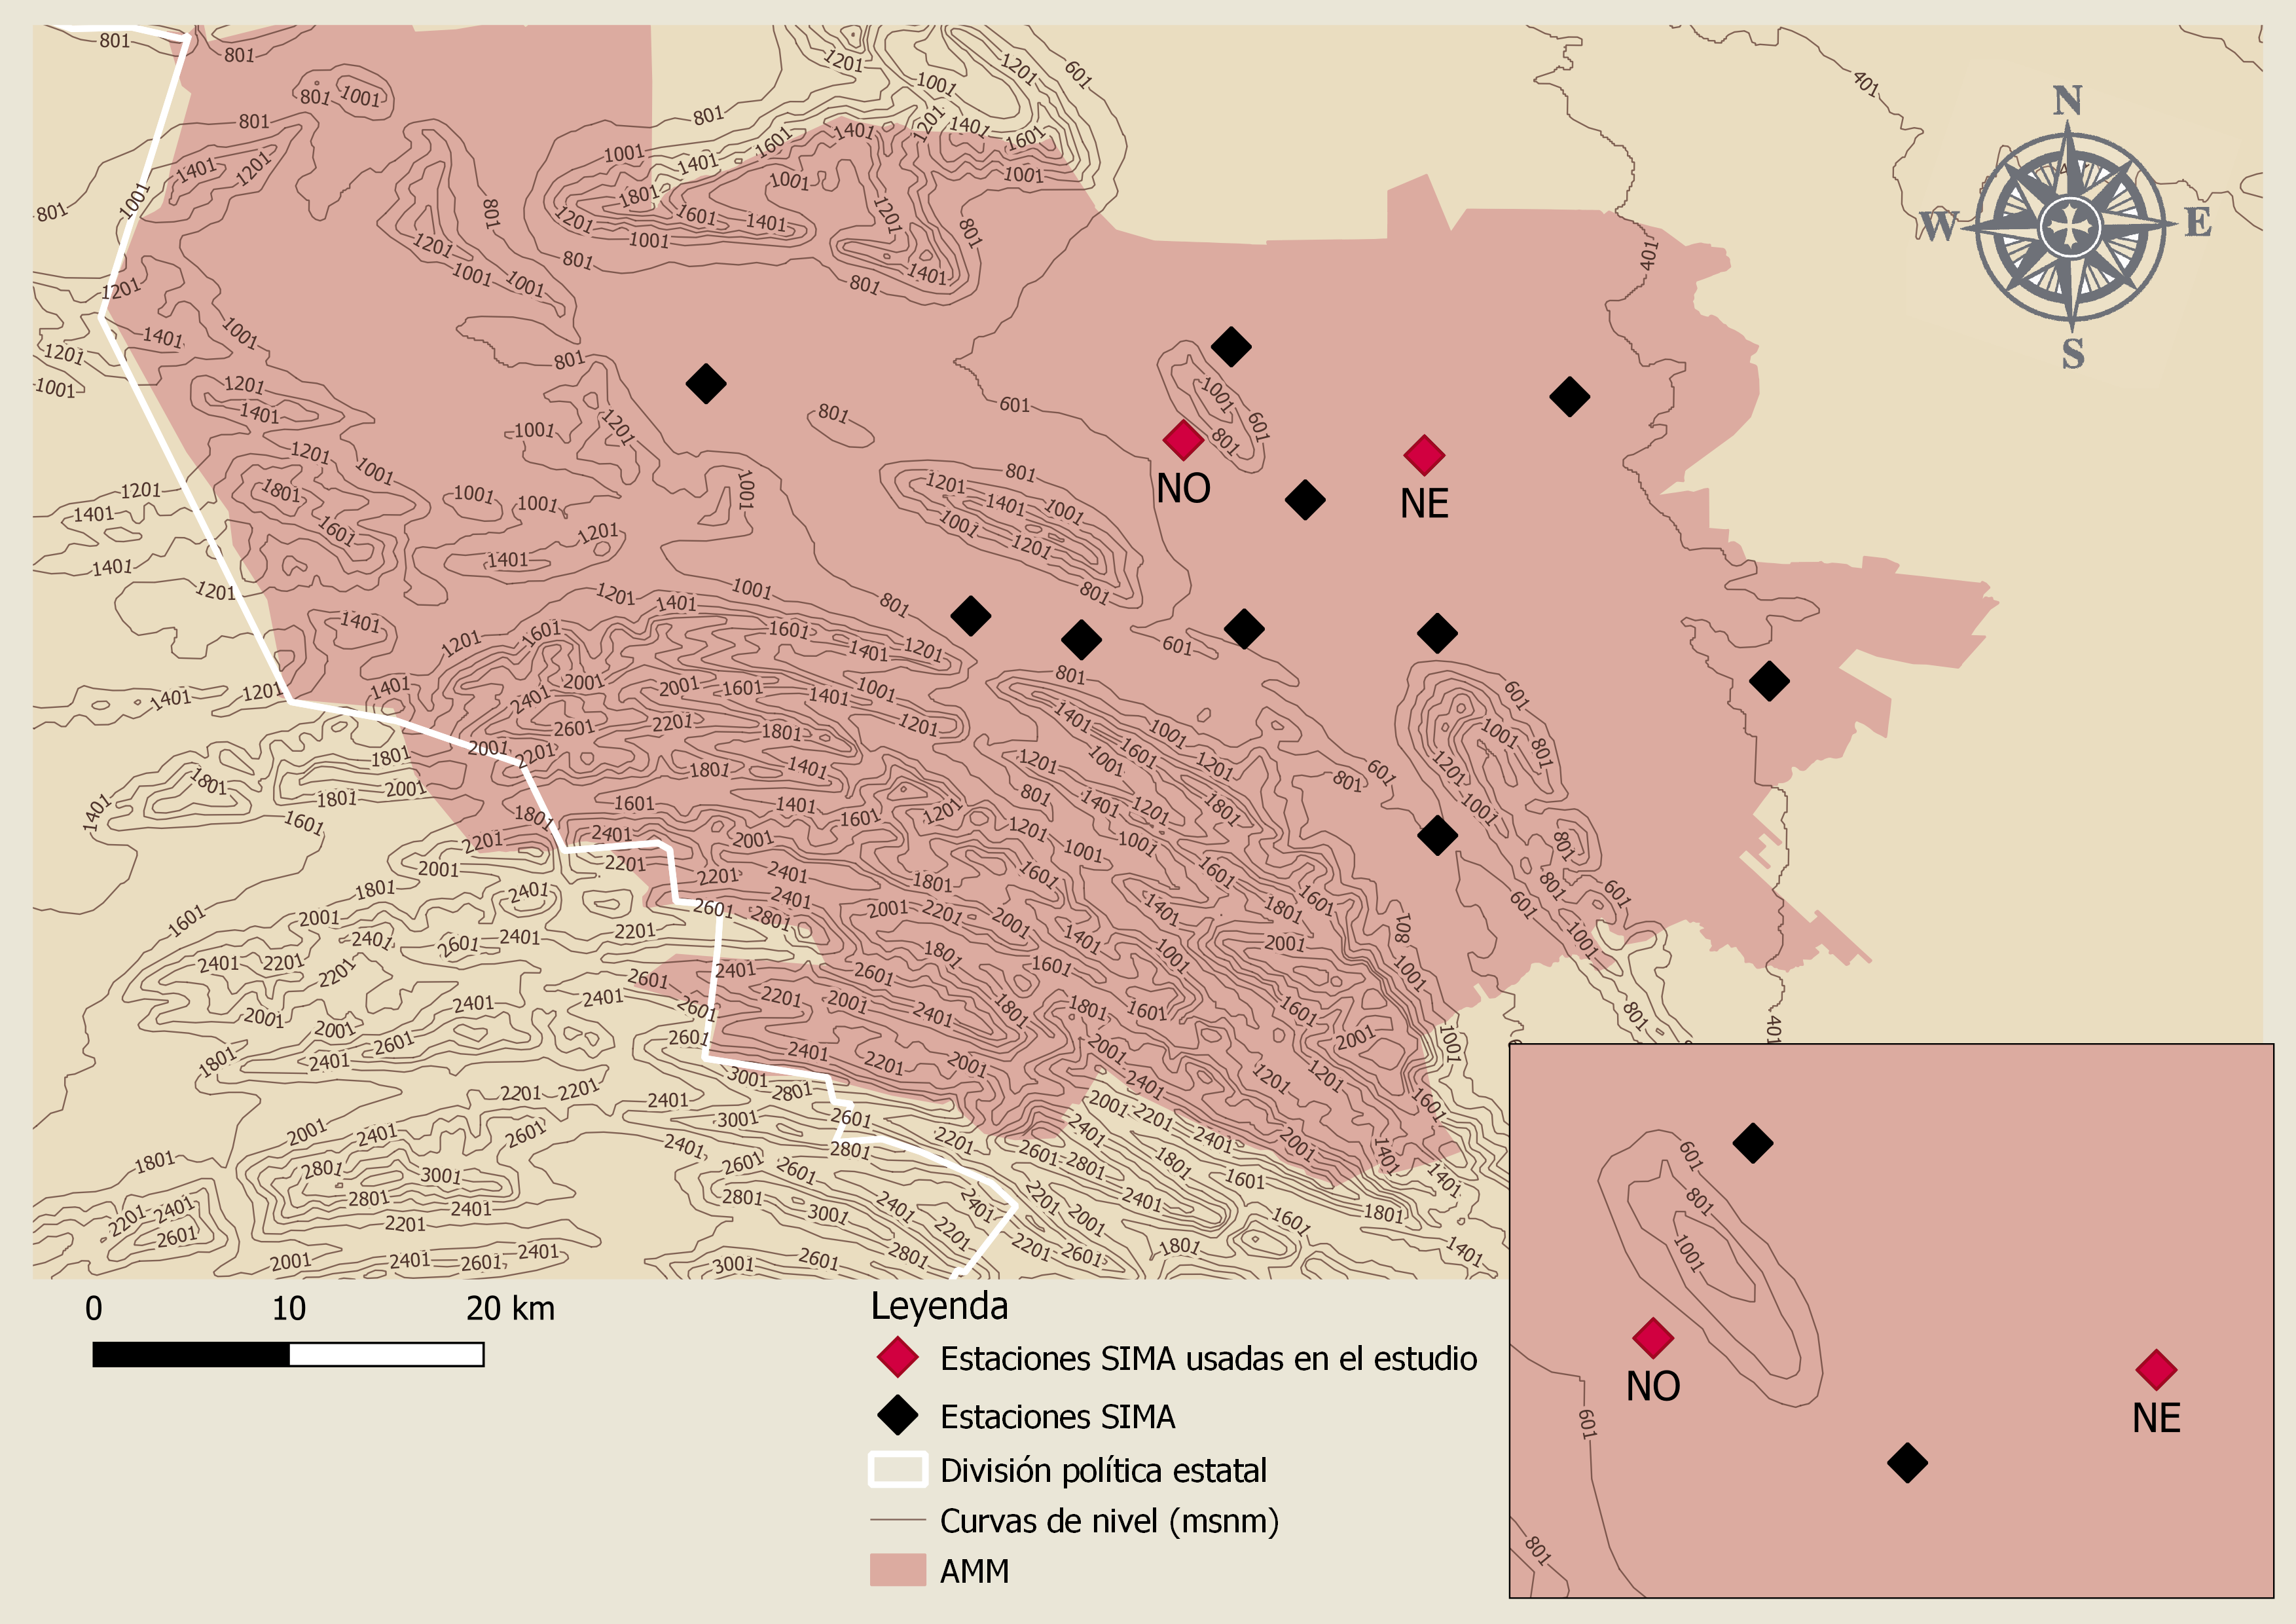
\includegraphics[scale=0.29]{images/AMM10.png}
\caption{Área Metropolitana de Monterrey (AMM)}
\end{figure}
\end{minipage}
\begin{minipage}{0.60\linewidth}
    Los aerosoles son partículas suspendidas en la atmósfera que pueden ser de origen natural o antropogénico. 
    La concentración de partículas de tamaño menor a 10$\mu$m (PM\textsubscript{10}) es una medida útil en el control de la calidad del aire. 
    Los aerosoles dependiendo su composición y tamaño provocan cambios en la climatología del lugar así como efectos nocivos en la 
    salud humana (principalmente problemas respiratorios). El Área Metropolitana de Monterrey (AMM) se ubica en una región montañosa 
    donde se realizan extracciones de material para la construcción (Pedreras) a la par de actividades industriales y alto flujo 
    vehicular. En este trabajo se presenta una estimación del Espesor Óptico de Aerosol a 550nm (AOD\textsubscript{550nm}) derivado del modelo SMARTS, 
    tomando como referencia la irradiancia solar global medida por las estaciones Noreste (NE) y Noroeste (NO) del Sistema Integral de 
    Monitoreo Ambiental (SIMA) de Nuevo León. 
    Estos resultados se comparan con las mediciones PM\textsubscript{10} en dichas estaciones a fin de contribuir al entendimiento de esta variable.
\end{minipage}
\begin{center}
\begin{shaded}
\textbf{\textcolor{ver}{Metodología}}
\end{shaded}
\end{center}
\begin{minipage}{0.75\linewidth}
Se seleccionaron sólo las mediciones de radiación solar bajo cielo despejado. Se modificó el código fuente del modelo 
SMARTS para ingresar los valores de la Tabla \ref{tabla:parametros} y realizar iteraciones con el AOD\textsubscript{500nm}, 
hasta que la diferencia relativa entre la irradiancia medida y modelada alcanza el 10\% al mediodia solar.
\begin{table}[H]
    \changefontsizes{9.5pt}
        \centering
    \begin{tabular}{|c|c|c|c|c|c|c|c|c|c|c|c|c|c|c|} \hline
         \multirow{2}{*}{Estación} & \multirow{2}{*}{Lat}& \multirow{2}{*}{Lon} & \multirow{2}{*}{m snm} & CH\textsubscript{2}O & CH\textsubscript{4}& CO & HNO\textsubscript{2} & HNO\textsubscript{3} & NO & NO\textsubscript{2} & NO\textsubscript{3} & SO\textsubscript{2} & CO\textsubscript{2}&O\textsubscript{3}\\ \cline{5-15}
                &       &   &  & \multicolumn{10}{c|}{ppmv}  & \multicolumn{1}{c|}{DU} \\ \hline
       Noreste &  25.74&-100.26&476   & \multirow{2}{*}{0.007} & \multirow{2}{*}{0.3}& \multirow{2}{*}{0.35}    &   \multirow{2}{*}{0.002}  &  \multirow{2}{*}{0.005} & \multirow{2}{*}{0.2} & \multirow{2}{*}{0.02} & \multirow{2}{*}{5x10$^{-5}$}  &\multirow{2}{*}{0.05} & \multirow{2}{*}{390}&OMI\\
        Noroeste &  25.76&-100.46&571  &  & & & &  &  &  & &  & & NASA\\\hline
    \end{tabular}
    \caption{ Parámetros de entrada en modelo SMARTS: coordenadas geográficas de las estaciones Noreste y Noroeste,
    en un escenario de contaminación ’moderada’ (opción definida en el modelo) y medición de la columna de ozono (DU) por OMI-NASA}
    \label{tabla:parametros}
\end{table}
\end{minipage}
\begin{minipage}{0.25\linewidth}
    \begin{figure}[H]
        \centering
    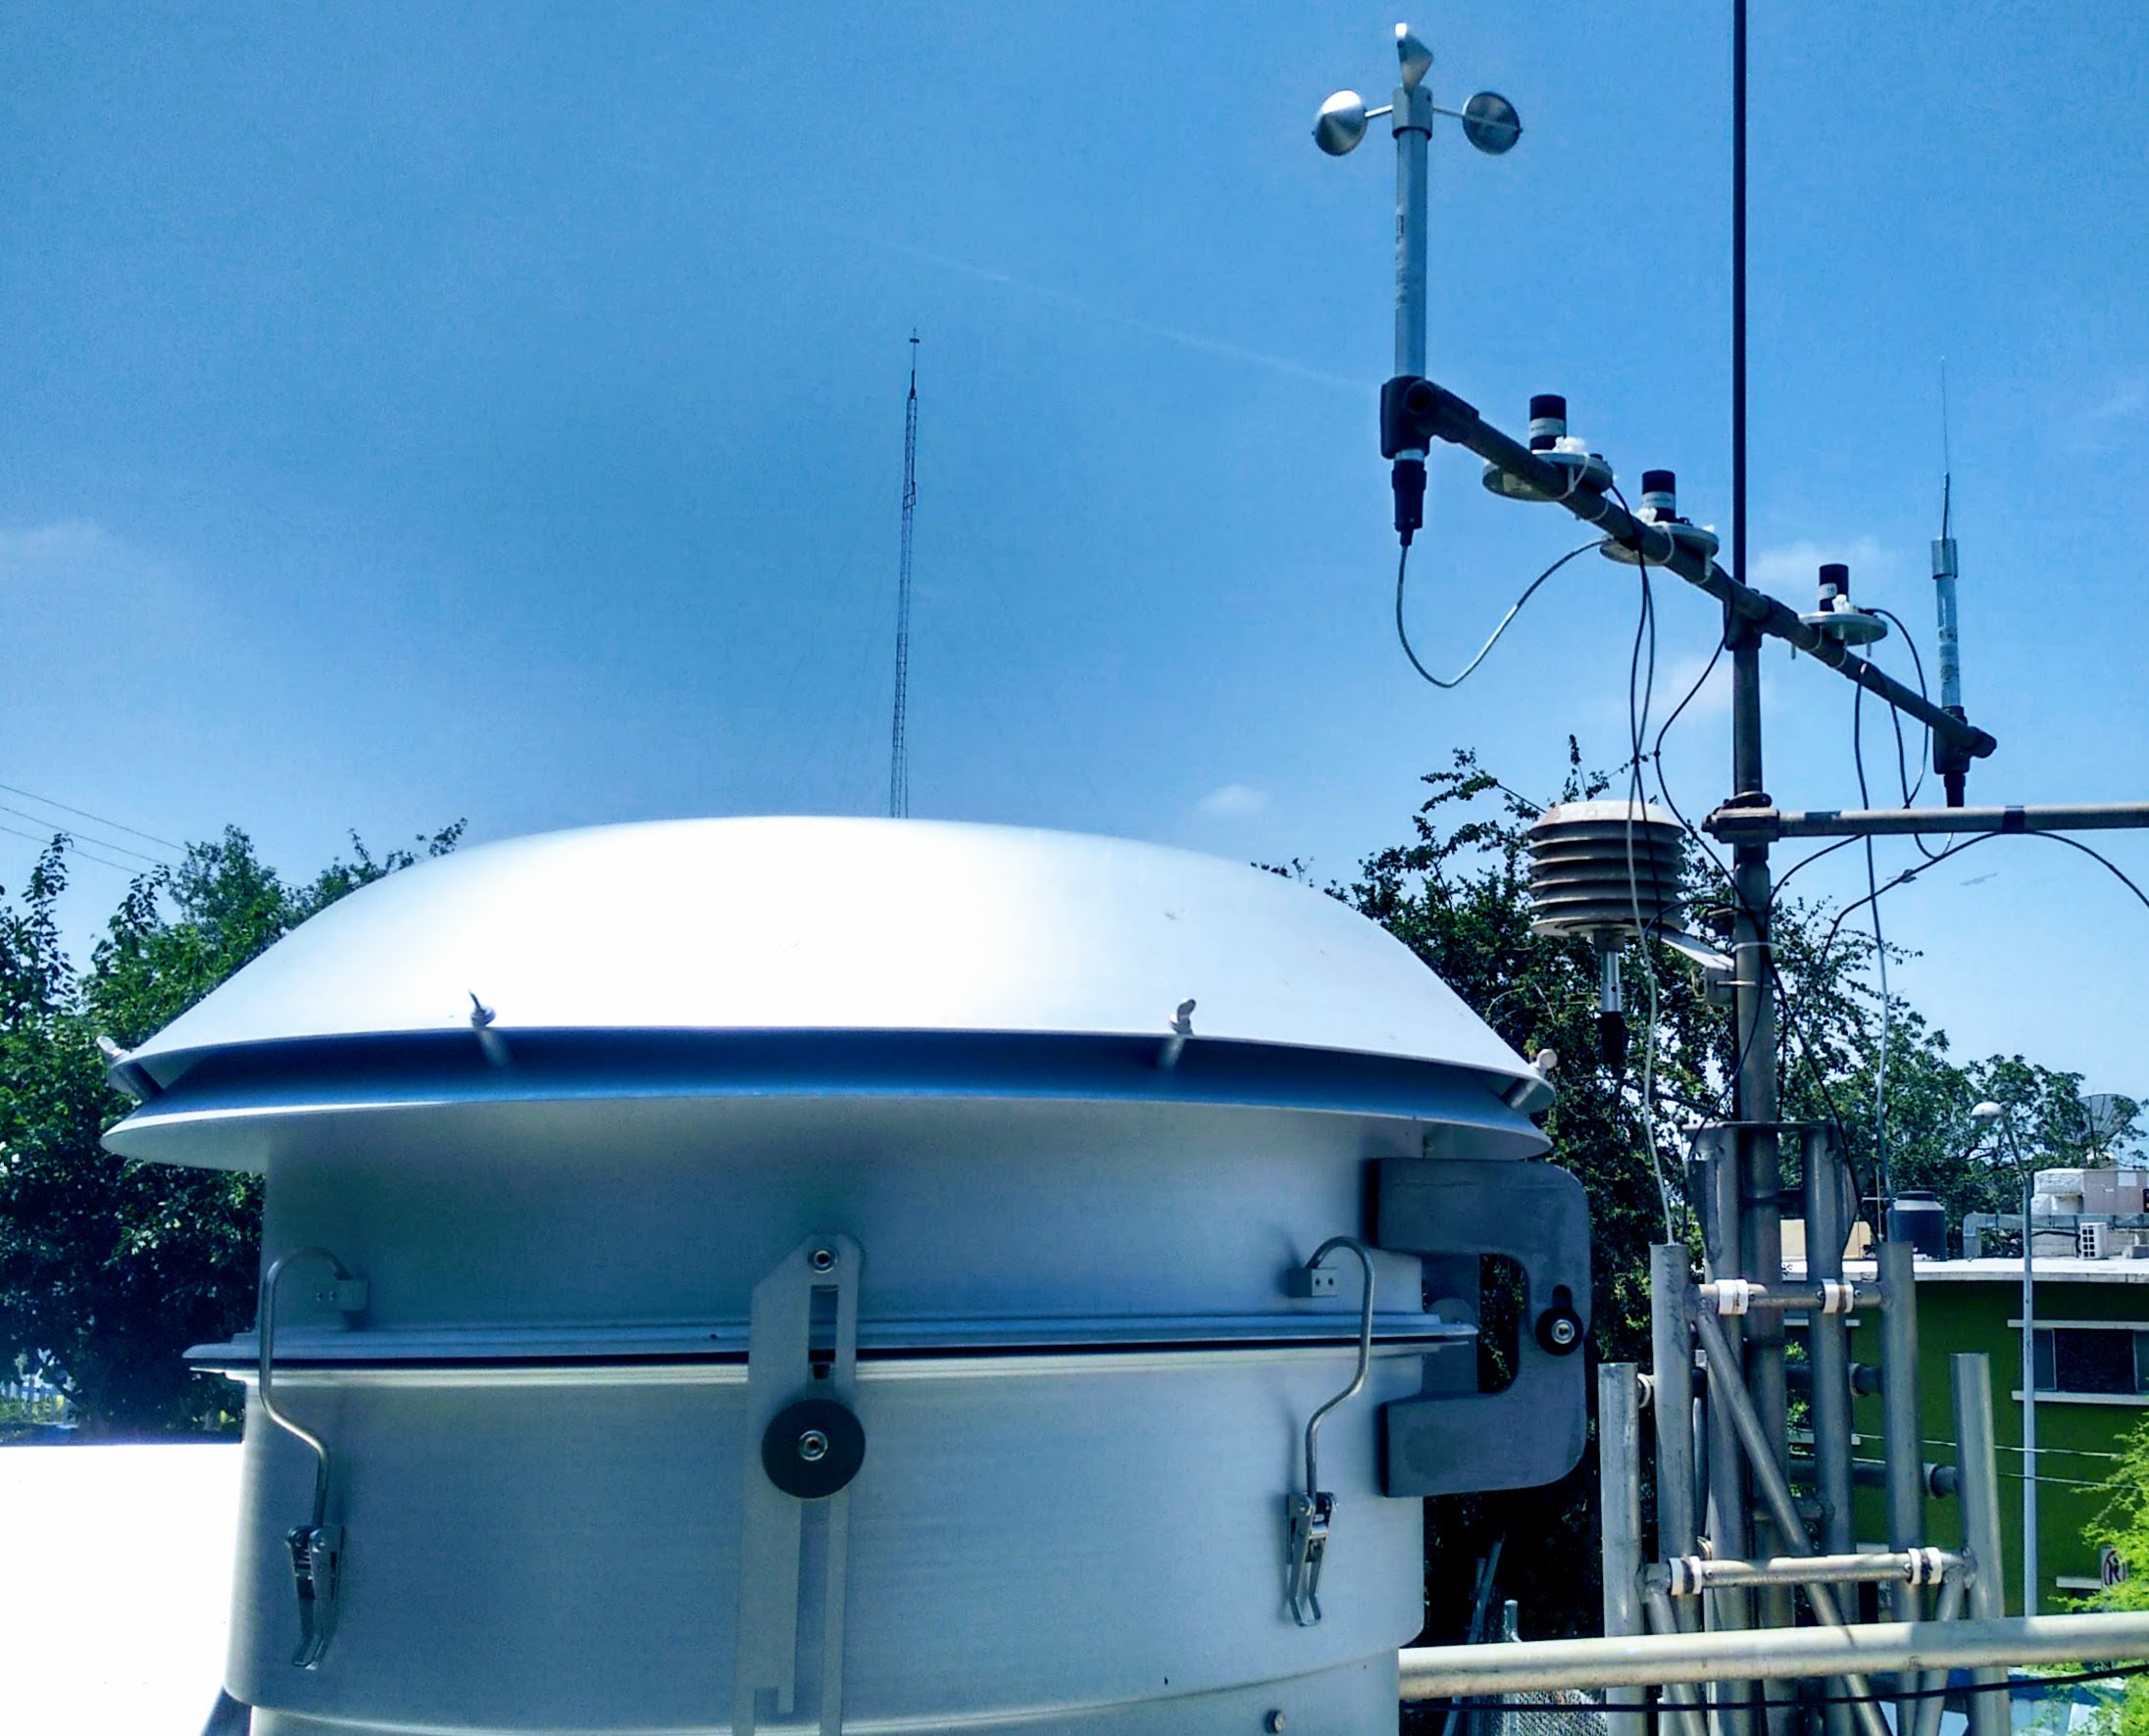
\includegraphics[scale=0.06]{images/mediciones.jpg}
    \caption{ Instrumento de medición de PM\textsubscript{10} perteneciente al SIMA}
    \end{figure}
\end{minipage}
\begin{center}
\begin{shaded}
\textbf{\textcolor{ver}{Resultados}}
\end{shaded}
\end{center}
\vspace{-0.8cm}
\begin{center}
    \begin{figure}[H]
        \centering
        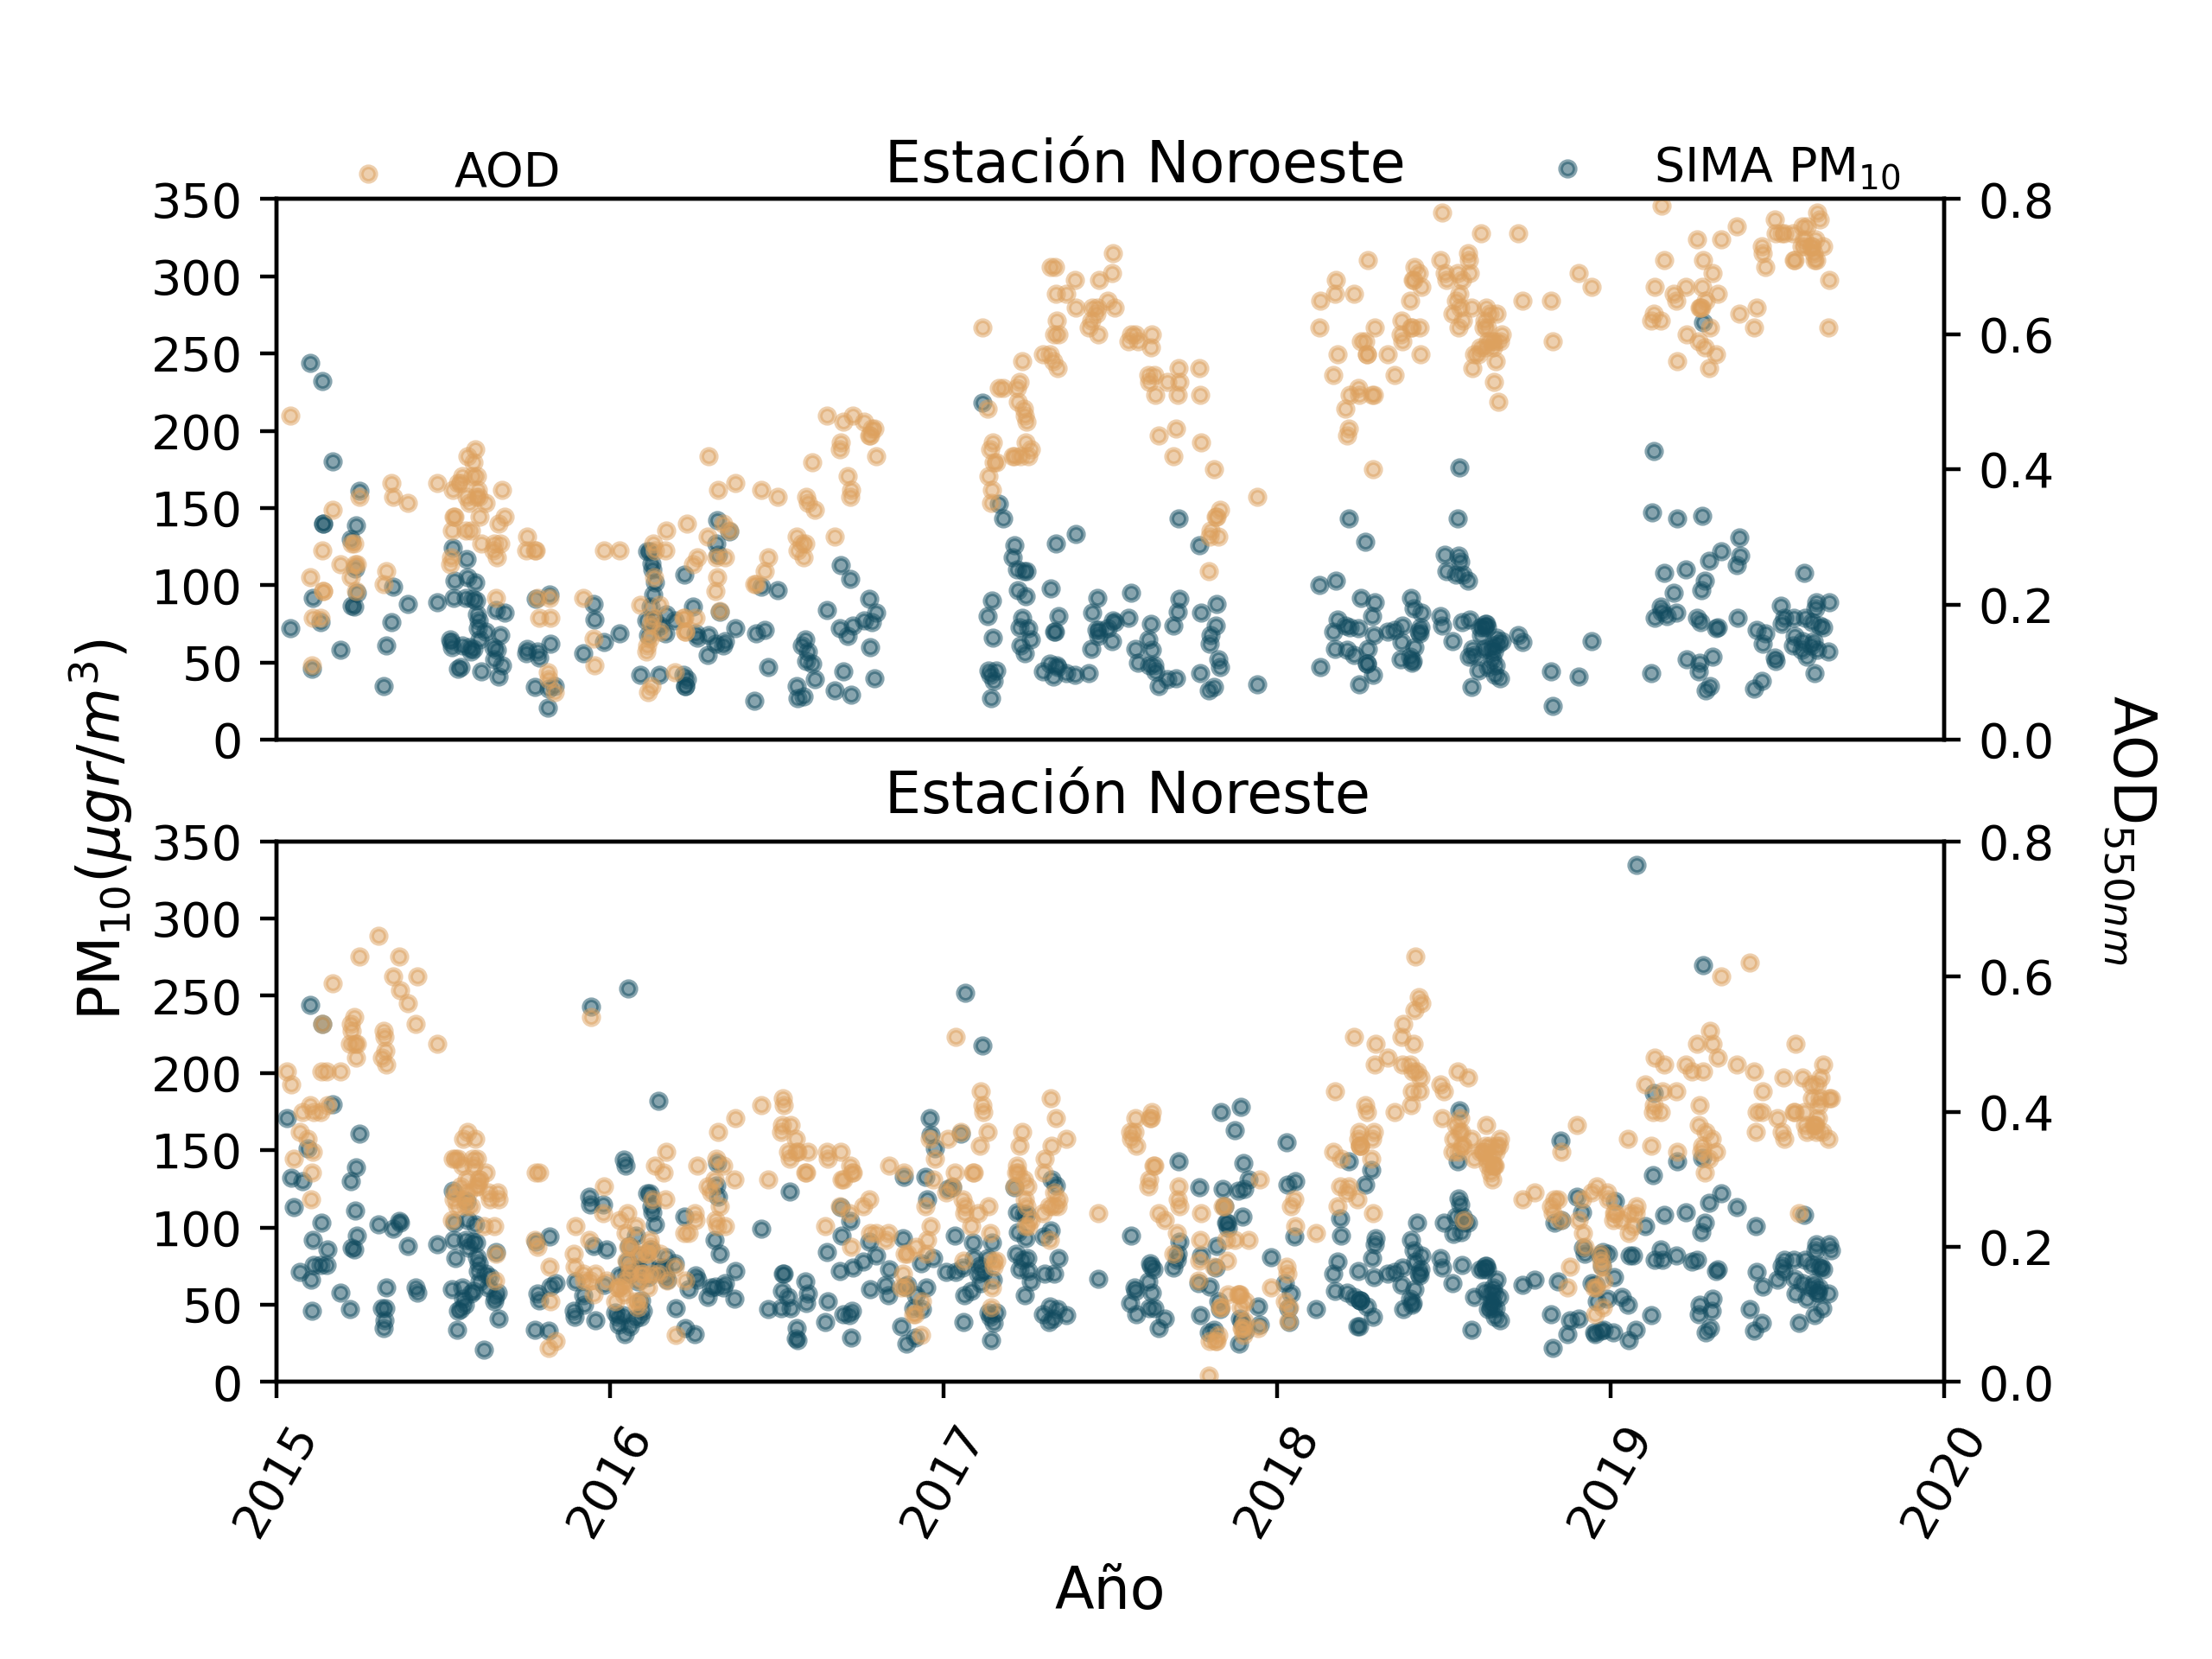
\includegraphics[height=8cm]{images/AODsandPM10.png}
        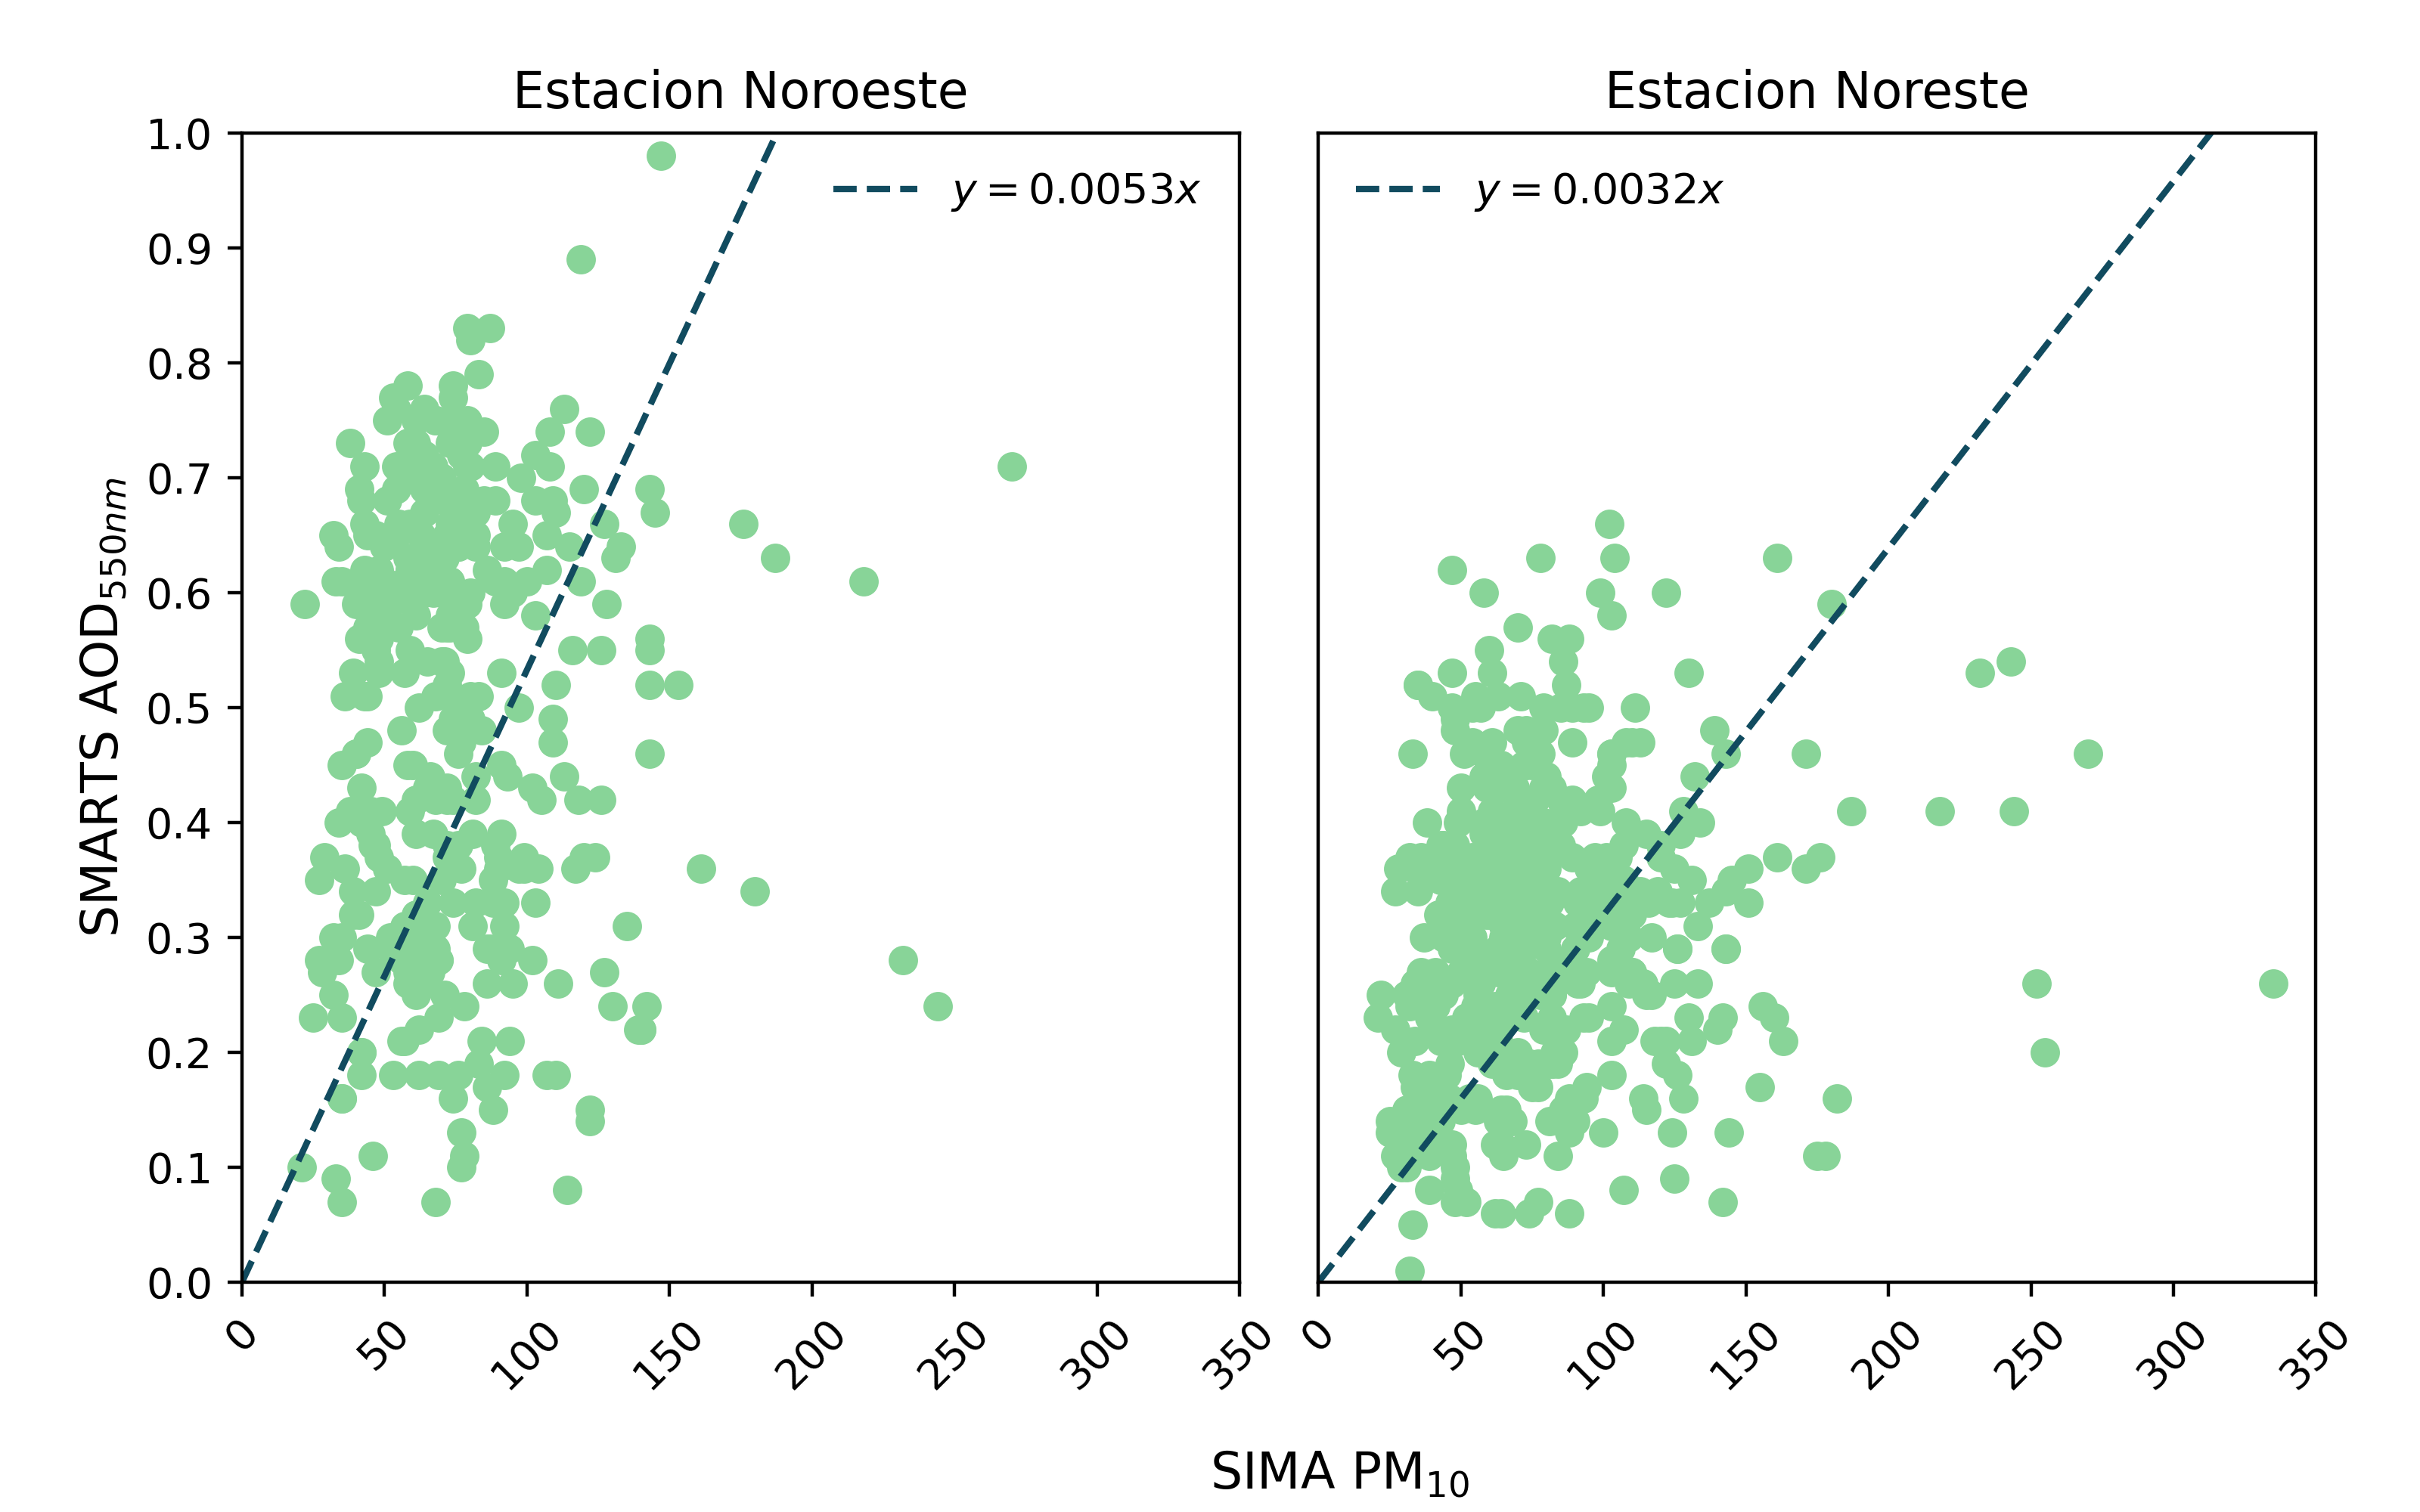
\includegraphics[height=7.7cm]{images/AODvsPM10.png}
        \caption{AOD\textsubscript{550nm} (círculos naranjas) derivado del modelo SMARTS y PM\textsubscript{10} (círculos azules) 
        medido por SIMA para las estaciones NO y NE (izq). Ajuste lineal del AOD\textsubscript{550nm} al medio día solar obtenido con SMARTS
        y el PM\textsubscript{10} medido en las estaciones SIMA, al mediodía solar en días de cielo despejado en el periodo 2015-2019 (der).}
    \end{figure}
\end{center}
\begin{minipage}{0.70\linewidth}
\begin{center}
\begin{shaded}
\textbf{\textcolor{ver}{Conclusiones}}
\end{shaded}
\end{center}
\begin{itemize}
    \item En la estación Noroeste existe una tendencia creciente en el AOD\textsubscript{550nm} posiblemente debido a un incremento en la actividad de la industria
    pedrera, aunado a la erosión progresiva del suelo los ultimos años. Los valores de PM\textsubscript{10} corresponden a mediciones a nivel del suelo que, debido a la altura,
     la circulación del viento y la presencia de un relieve irregular en la zona, pudieran originar una diferencia respecto al AOD\textsubscript{550nm} estimado.
     \item En los alrededores de la estación Noreste hay una mayor diversidad de actividades industriales
     así como tráfico vehicular en comparación con la estación Noroeste además de un relieve uniforme. Por lo tanto, los aerosoles que
     circulan podrían ser producidos por actividades antropogénicas de rutina, es por ello que se mantiene una tendencia
      semejante a la del PM\textsubscript{10} medido.
\end{itemize}
\end{minipage}
\hspace{0.8cm}
\begin{minipage}{0.25\linewidth}
\vspace*{-0.6cm}
\begin{center}
\begin{shaded}
\textbf{\textcolor{ver}{Referencias}}
\end{shaded}
\end{center}
\begin{enumerate}
    \item Kaufman, Y. J., et al., Nature, (419) 215 – 223, 2002.
    \item Ipiña A, Salum GM, Crinó E, Piacentini R, Adv in Space R 966–977, 2012.
    \item Wang J and Sundar AC. Geophysical Research Letters (30) 21-2095, 2003
\end{enumerate}
\end{minipage}
\end{document}